\chapter{Implementation}

This chapter covers the following topics:
\begin{enumerate}
\item concepts in Elektra that are relevant for this thesis
\item the plugins and enhancements we contributed to Elektra
\end{enumerate}


\section{Elektra Concepts}\label{elektra-plugins}

Before we elaborate the contributions that were made to Elektra during the writing of this thesis, we need to explain some internal concepts of Elektra.

\subsection{Key and Keyset}

Elektra abstracts configuration settings in a hierarchical key-value database.
A \emph{keyset} holds zero or more keys.
The \emph{key} represents a configuration value within the configuration setting and holds:
\begin{enumerate}
\item its path within the configuration hierarchy
\item its configuration value either as a string value or as a binary value
\item optionally its meta-keys, which are keys that further describe the key itself
\end{enumerate}

Elektra uses meta-keys for different purposes:

\begin{enumerate}
\item state information of the key (for example: encrypted, encoded, ...)
\item data validation (for example: numeric value, binary value, ...)
\item formatting (for example: position in file, number of spaces between parameters, ...)
\end{enumerate}

In order to avoid ambiguity we do not use Elektra's terms in this thesis.
We refer to a \emph{configuration setting} rather than to a \emph{keyset}.
We refer to \emph{configuration values} rather than to Elektra \emph{keys}, in order to avoid confusion with cryptographic \emph{keys}.
From now on if we refer to a \emph{key}, we mean a \emph{cryptographic key}.

\subsection{Plugin}\label{impl_elektra_plugin}

The core of Elektra is kept small, meaning that it provides mainly the database abstraction as well as a plugin system.
All the configuration access operations are performed by plugins.\cite{raab2010thesis}
Every plugin should fulfill exactly one purpose.
This design decision was inspired by the UNIX philosophy.
Let us illustrate what plugins can do by giving some examples:
\begin{enumerate}
\item the \crypto ~encrypts and decrypts configuration values
\item the \base ~encodes and decodes binary values to and from Base64 strings
\item the \texttt{ini} plugin reads from and writes to ini files
\end{enumerate}

Plugins can be divided into two categories:
\begin{enumerate}
\item filter plugins
\item storage plugins
\end{enumerate}

A \emph{filter plugin} modifies configuration values before they are written to a file or after they have been read from a file.
A \emph{storage plugin} directly reads from or writes to a configuration file.

A plugin can export different methods in order to fulfill its purpose.
They are enumerated below:

\subsubsection{checkconf}\label{impl-method-checkconf}

At this method a plugin may validate the backend configuration as well as
the plugin configuration. The plugin may modify the configuration or
report that the configuration is incomplete or wrong in some way.

We added this method during the writing of this thesis.
Its introduction was neccessary for the development of the \crypto ~as well as the \fcrypt.

\subsubsection{open}\label{open}

The \texttt{open} method is called to initialize the plugin.

\subsubsection{close}\label{close}

The \texttt{close} method is called to properly shutdown the plugin and
release all resources it may hold.

\subsubsection{set}\label{set}

For storage plugins the \texttt{set} method is called when changes made to the key-value
database should be persisted.
Filter plugins export this method to modify the keyset (for example: encode binary values using the Base64 schema).

\subsubsection{get}\label{get}

The \texttt{get} method is called when the content of the key-value
database is requested by an application.
Filter plugins provide this method to transform data in the keyset (for example: decoding Base64 encoded strings back into their corresponding binary value).
Storage plugins typically perform read operations within this method.

\subsection{Elektra State Sequence}

First Elektra calls \texttt{open} and changes its state to ``opened''.
Afterwards Elektra can either be closed by a \texttt{close} call or the configuration can be read by calling \texttt{get}.
After the first call of \texttt{get} Elektra is ``ready''.
Now the configuration held by Elektra may be modified with a call of \texttt{set} or the data may be read again by calling \texttt{get}.
After all \texttt{get} and \texttt{set} calls are done, Elektra is closed by a call of \texttt{close}.\cite{elektra-doc}

Figure \ref{impl_elektra_states} on page \pageref{impl_elektra_states} illustrates how the states in Elektra change by the calls of the methods mentioned above in Section \ref{impl_elektra_plugin} on page \pageref{impl_elektra_plugin}.

\begin{figure}[h]
\center
\caption{State changes in Elektra}
\label{impl_elektra_states}
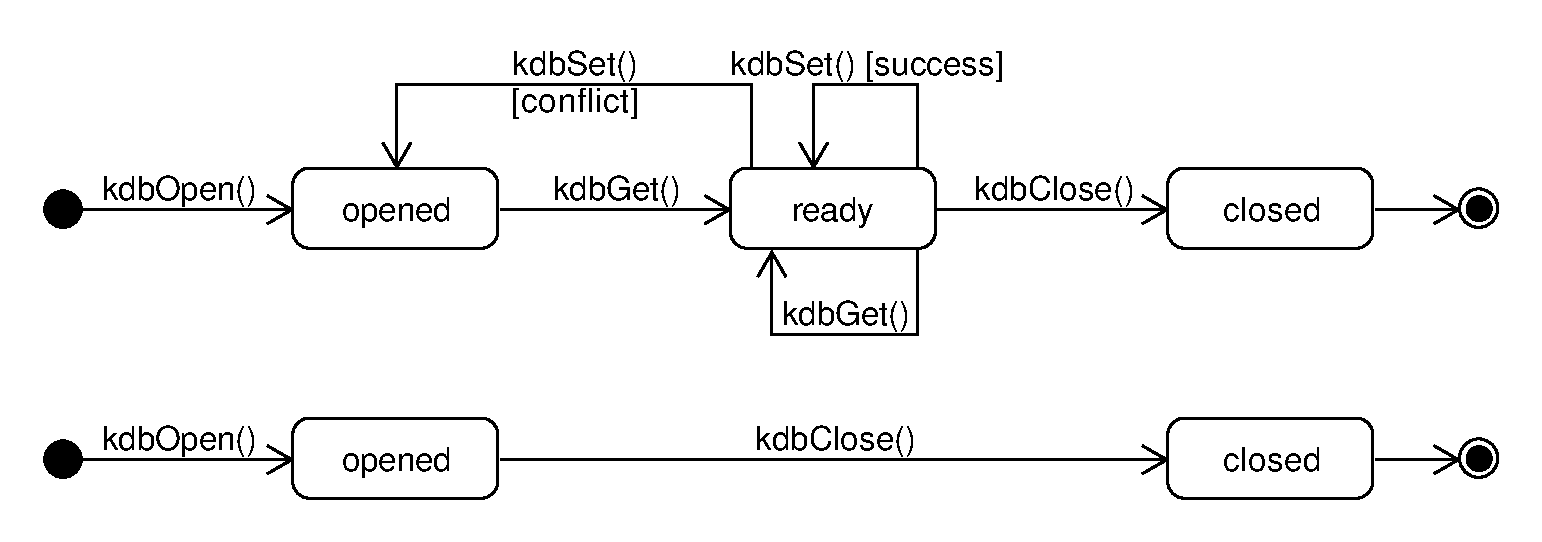
\includegraphics[width=15.0cm]{umlet-figures/impl_elektra_state.pdf}
\end{figure}

\subsection{Backend}

Backends are one or more plugins combined into a unit that interact with a single configuration file.
The backend is mounted into Elektra's configuration hierachy.
This process is similar to the mounting process in UNIX-like file systems, where a device can be mounted to a specific directory in the virtual file system.
In terms of Elektra the virtual file system is the key-value database and the device is the configuration file.
Every backend has its own configuration itself (i.e. backend configuration), which specifies the runtime behavior of the plugins within the backend.

\subsection{Compilation Variants}

Elektra's build scripts provide a functionality called \emph{compilation variants}, which means a plugin is being compiled multiple times with minor differences.
Let us demonstrate this idea using the \crypto ~as an example.
Cryptographic functions are provided by different libraries (see Section \ref{intro-provider} on page \pageref{intro-provider}) interchangeably.
The basic structure of the plugin stays the same for every compilation variant except for the library-specific calls.
These calls are encapsulated using C preprocessor directives, which form the actual compilation variants.
Listing \ref{impl-cryptoInit} on page \pageref{impl-cryptoInit} further illustrates the use of compilation variants, showing how the crypto libraries are initialized by the \crypto.

\begin{lstlisting}[label=impl-cryptoInit,language=C,caption={Example of how to use compilation variants in Elektra}]
static int elektraCryptoInit (Key * errorKey)
{
#if defined(ELEKTRA_CRYPTO_API_GCRYPT)
	return elektraCryptoGcryInit (errorKey);
#elif defined(ELEKTRA_CRYPTO_API_OPENSSL)
	return elektraCryptoOpenSSLInit (errorKey);
#elif defined(ELEKTRA_CRYPTO_API_BOTAN)
	return elektraCryptoBotanInit (errorKey);
#else
	return 1;
#endif
}
\end{lstlisting}

As we can see every crypto library is handled differently but the code frame of the plugin stays the same for all compilation variants.

\section{Crypto Plugin}\label{crypto-plugin}

\subsection{Reasons For Developing The Plugin}

In order to evaluate our research questions we need a reference application with a high degree of modularity.
The modularity is required to gain profound insight in the runtime behavior of the reference application.
By combining different Elektra plugins we can test a variety of possible use cases.

Elektra originally did not provide any cryptographic functions when we started working on this thesis.
So we choose to develop the \crypto ~for Elektra.
The \crypto ~enables us to use Elektra as benchmark environment.

\subsection{Benefits For The Elektra Project}

Elektra is a configuration database and as such it will be used for storing sensitive configuration values (for example: login credentials) at some point.
Leaving these values unencrypted is a security threat.
The \crypto{} is a way of tackling this threat by providing transparent encryption and decryption.
This means that the configuration values are stored encrypted on the filesystem and are decrypted by Elektra whenever the application requests its configuration.
Thus the encryption and the decryption work transparent to both the user and the application.
The \crypto{} can simply be added to a backend and thus integrates well with other Elektra plugins.

\subsection{Challenges}

The first challenge was to design the \crypto ~in a way that supports more than one provider of cryptographic functions.
With the goal of comparability in mind, the encryption and decryption schema will be similar for each provider.
Otherwise no conclusions can be drawn from differing benchmark results.
Elektra's compilation variants enable the support for multiple providers.
For every provider we want to integrate, a new compilation variant is added to the \crypto.

The next problem was how to generate, derive and restore the keys for the cryptographic functions.
This part of the plugin is crucial from a security perspective.
Any kind of wrongdoing in this module could lead to leaks, endangering the confidentiality of the protected data.
The first design that came to mind was a password based schema that utilizes the Password-Based Key Derivation Function 2 (PBKDF2).\footnote{PBKDF2 is specified in RFC 2898.}
However, this approach is not suitable for any kind of batch operation as the program flow would be interrupted to ask for a password input.
So we decided to delegate the handling of cryptographic keys to an existing key store: GnuPG.
GnuPG in combination with the \texttt{pinentry} utilities turned out to be a great way of managing keys.
In addition the users benefit from this approach because they can simply use their existing PGP keys and even smart-cards for securing their data in Elektra.

In the following section we are going to dive deeper into the technical details of the implementation of the \crypto.

\subsection{Technical Aspects}

The \crypto{} acts as a filter that is applied to the configuration setting before the storage plugin reaches its \texttt{kdb set} phase.
Later on, when the encrypted configuration is requested, the plugin decrypts the configuration setting after the storage plugin read the configuration file in its \texttt{kdb get} phase.
Figure \ref{impl_crypto_overview} on page \pageref{impl_crypto_overview} further illustrates how the process works.

\begin{figure}[h]
\center
\caption{Crypto Plugin: Overview of the encryption and decryption process}
\label{impl_crypto_overview}
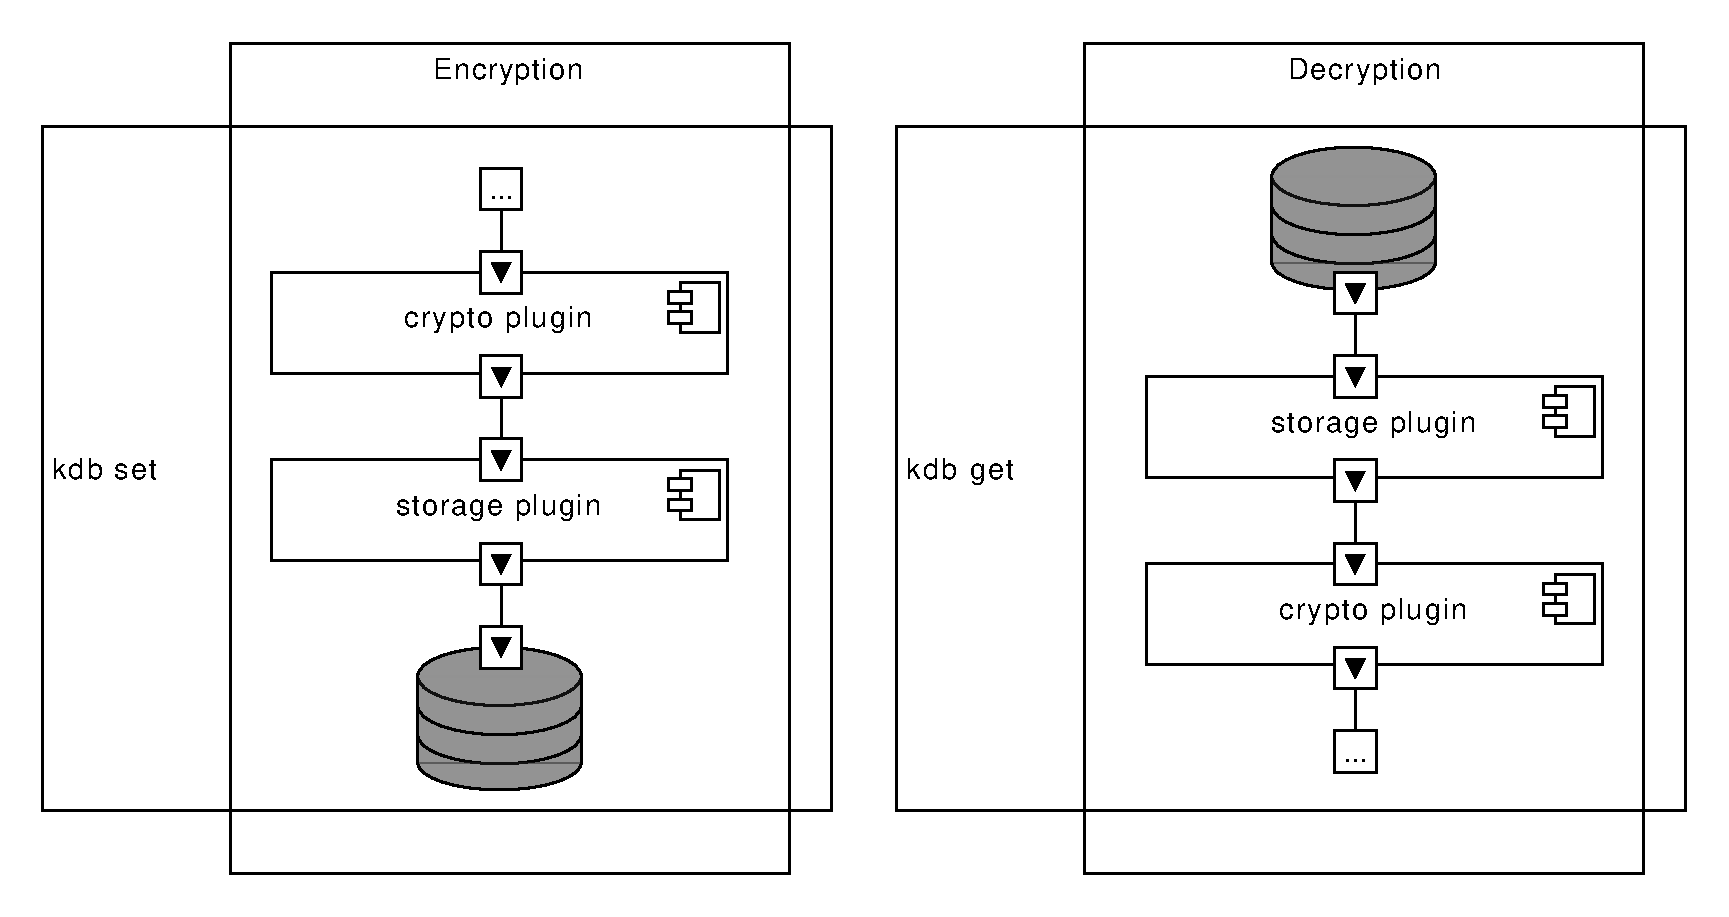
\includegraphics[width=15.0cm]{umlet-figures/impl_crypto_overview.pdf}
\end{figure}

Not all configuration values in the configuration setting are considered for encryption or decryption.
The \crypto{} uses a metakey to identify which configuration values have to be processed.
If a metakey with name \texttt{``crypto/encrypt''} is set to a value of \texttt{``1''} then the configuration value is marked for encryption.
The plugin checks the metakey and only encrypts values if the metakey is set properly.
The decryption works analogous.
All other configuration values, which are not marked, are ignored and left unchanged by the \crypto.

\subsection{Cryptographic Details}

In this section we elaborate the details of how the encryption and decryption process works.

\subsubsection{Data Structures}

The \crypto ~defines a single data structure, which is propagated throughout the plugin:

\paragraph{elektraCryptoHandle} is a structure that abstracts the library specific data types which hold keys and initialization data for the cryptographic functions.

Listing \ref{list-elektraCryptoHandle} on page \pageref{list-elektraCryptoHandle} shows the definition of the \texttt{elektraCryptoHandle} for the OpenSSL plugin variant.

\begin{lstlisting}[label=list-elektraCryptoHandle,language=C,caption={Definiton of elektraCryptoHandle for the OpenSSL crypto plugin variant}]
typedef struct
{
	EVP_CIPHER_CTX * encrypt;
	EVP_CIPHER_CTX * decrypt;
} elektraCryptoHandle;
\end{lstlisting}


\subsubsection{Message Structure}
\label{impl-msgstruct}

The \crypto{} operates on configuration values.
During its work it modifies the value as well as the meta-data.
The value is always transformed into binary data.
In order to restore the value to its original type during decryption, some header information has to be stored.

Table \ref{impl-msgheader} on page \pageref{impl-msgheader} shows the information which is encoded into the first cryptographic block during encryption.

\begin{table}[h]
\centering
\caption{Structure of the crypto message header}
\label{impl-msgheader}
\begin{tabular}{lrrlc}
	\textbf{element}           & \textbf{offset} & \textbf{length} & \textbf{data type}    & \textbf{encrypted} \\ \hline
	magic number ``\#!crypto'' & 0               & 8 B             & character             & no                 \\
	payload version            & 8               & 2 B             & character             & no                 \\
	length of the salt $L_S$   & 10              & 4 B             & unsigned long integer & no                 \\
	salt                       & 14              & $L_S$ B         & byte                  & no                 \\
	original data type         & 14 + $L_S$      & 1 B             & byte                  & yes                \\
	original content length    & 15 + $L_S$      & 4 B             & unsigned long integer & yes                \\ \hline
\end{tabular}
\end{table}

The salt is a sequence of random bytes and is used in cryptography to prevent table-based key guessing attacks.
The content length is saved because most provider of cryptographic functions do not support padding out of the box, which means that they always operate on whole blocks of data, where the block size depends on the cryptographic algorithm that is used.

\subsubsection{Key Derivation}

As mentioned before, GnuPG is used for managing the users' asymmetric keys.
GnuPG is executed to store and receive a \emph{master password}, which is a part of the plugin configuration of the \crypto.
Whenever a cryptographic key is required, the master password is fetched from the plugin configuration and decrypted.
Then the PBKDF2 is applied to the decrypted master password together with a salt, so that a cryptographic key as well as an initialization vector can be derived.

\subsubsection{Crypto Plugin Methods}

The \crypto ~implements Elektra's plugin methods (see Section \ref{impl-method-checkconf} on page \pageref{impl-method-checkconf}).
In the following section the program flow of the plugin methods is explained.

\paragraph*{open}
initializes the provider of cryptographic functions.

\paragraph*{close}
properly shuts down the provider of cryptographic functions.

\paragraph*{get}
The \texttt{get} method takes a configuration setting as input.
The \crypto ~iterates over the configuration setting and checks for every configuration value if it has been encrypted.
This is done by using the metakey mentioned before.
If the configuration value is encrypted, the \crypto ~decrypts it and thus restores the configuration value to the state it was in before the encryption took place.

Figure \ref{impl_decrypt} on page \pageref{impl_decrypt} illustrates how the \texttt{get} method works in detail.

\begin{figure}[h]
\center
\caption{Crypto Plugin: Decryption of a keyset at the kdb get method}
\label{impl_decrypt}
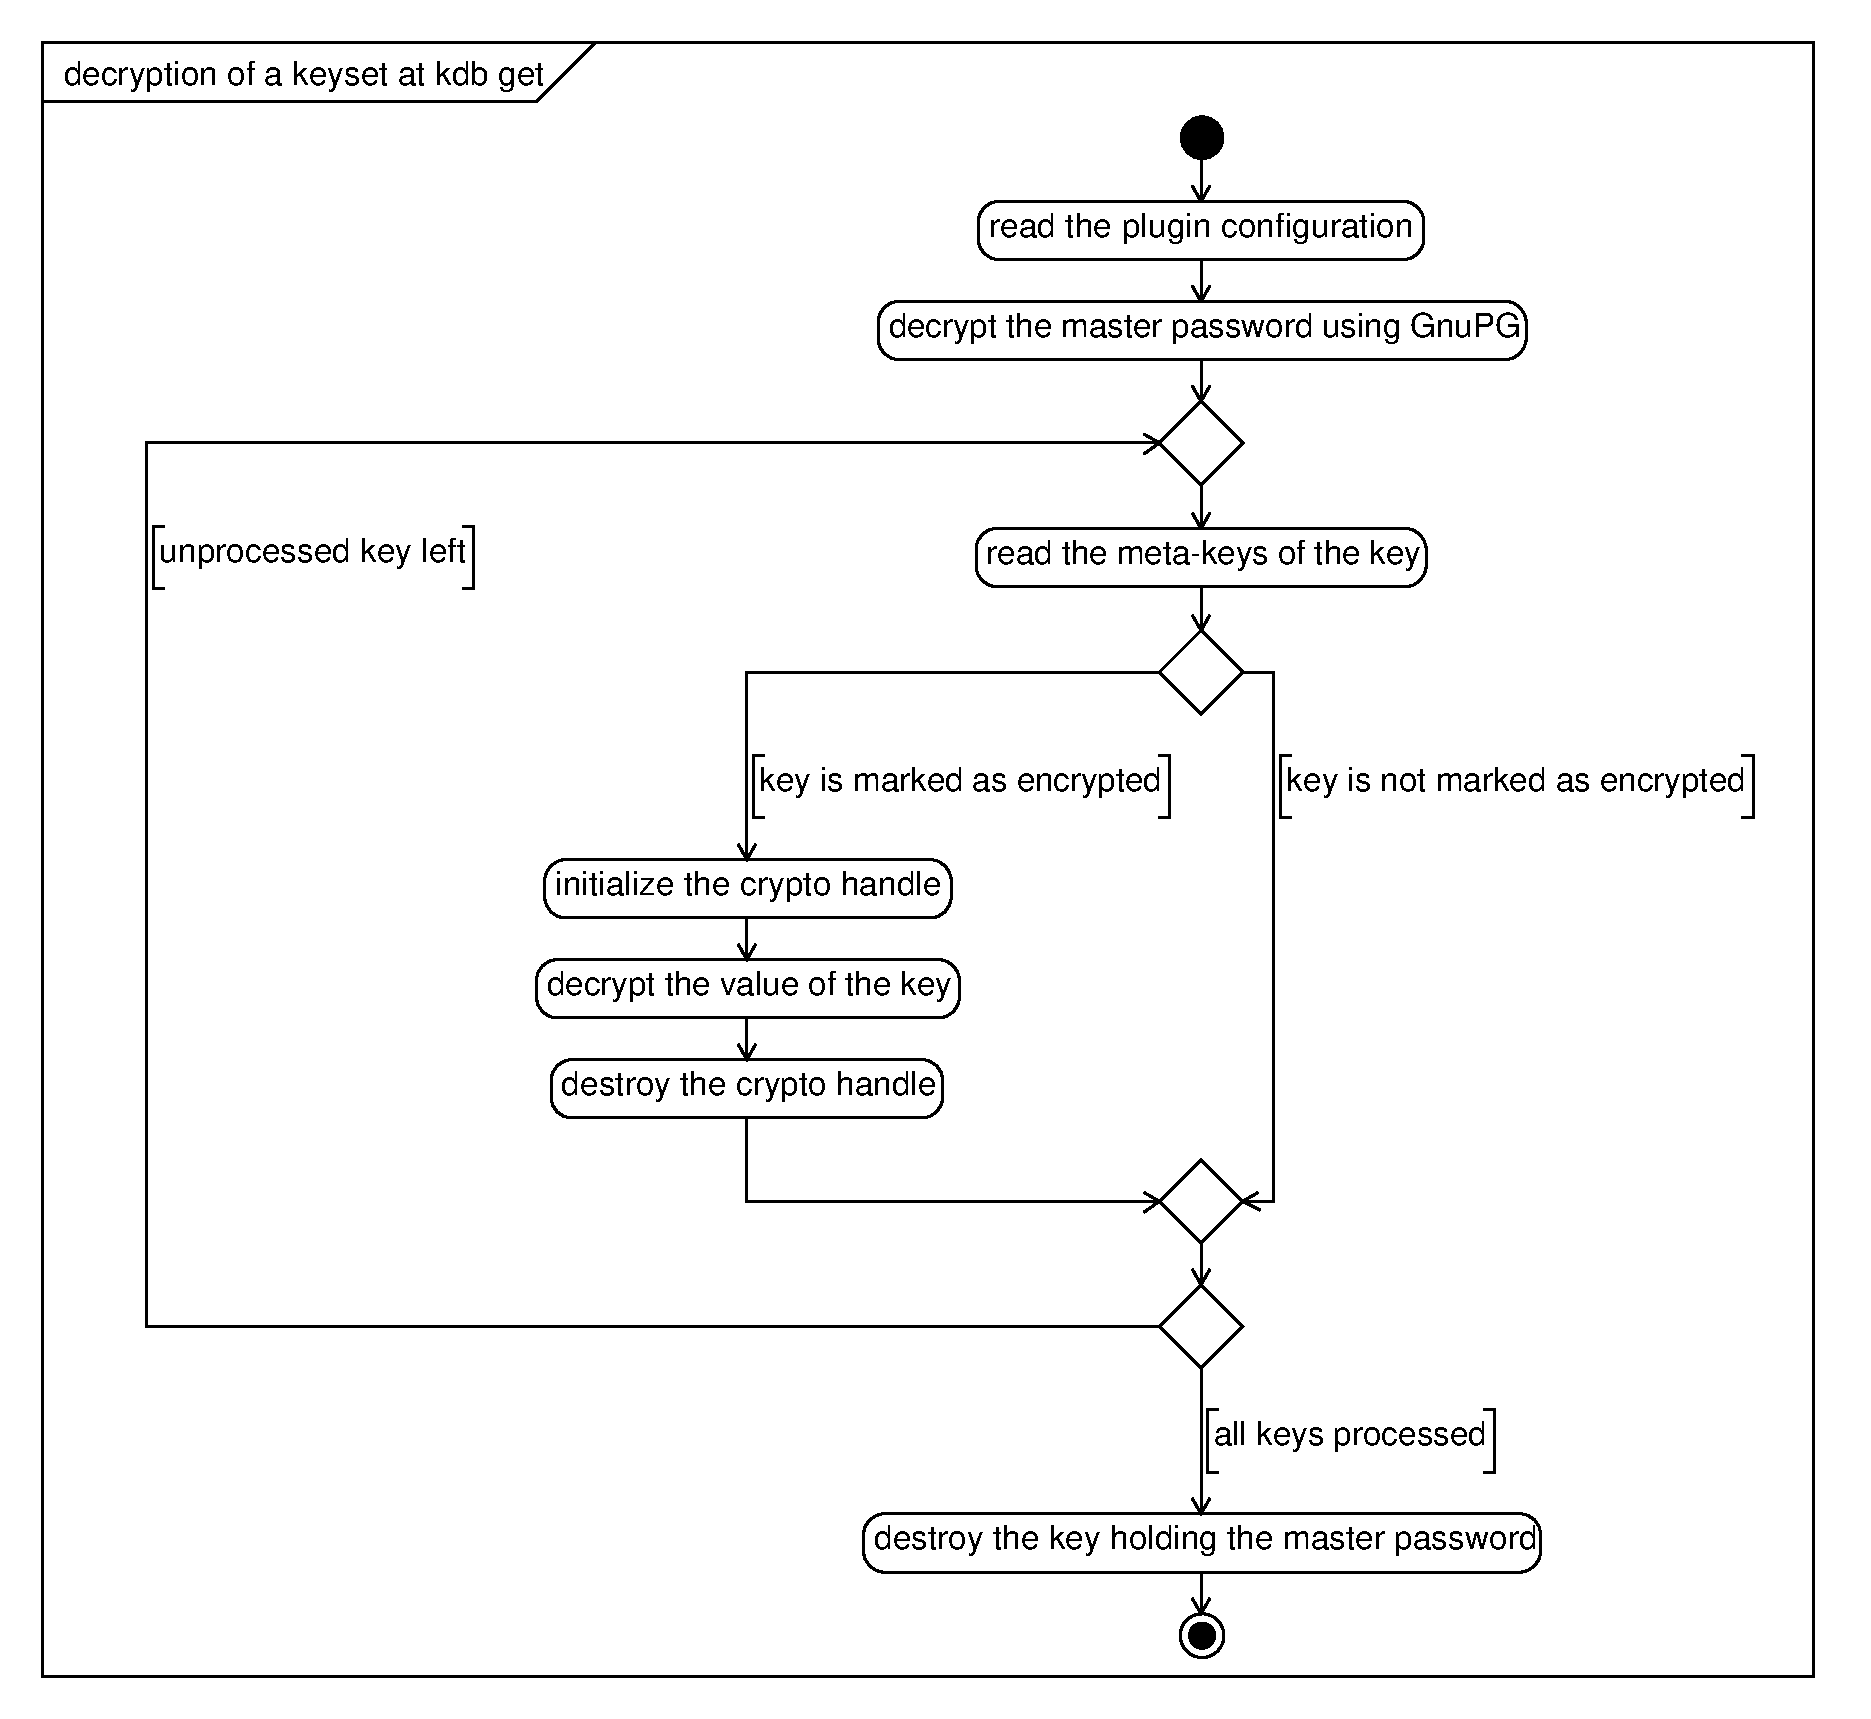
\includegraphics[width=15.0cm]{umlet-figures/impl_decrypt.pdf}
\end{figure}


\paragraph*{set}
The \texttt{set} method takes a configuration setting as input.
The \crypto ~iterates over the configuration setting and checks every configuration value if it has been marked for encryption.
Marking a configuration value for encryption is done by using a metakey.
If the metakey is present, the \crypto ~generates a message header (see Section \ref{impl-msgstruct} on page \pageref{impl-msgstruct}) including a random salt and encrypts the configuration value.

Figure \ref{impl_encrypt} on page \pageref{impl_encrypt} illustrates how the \texttt{set} method works in detail.

\begin{figure}[h]
\center
\caption{Crypto Plugin: Encryption of a keyset at the kdb set method}
\label{impl_encrypt}
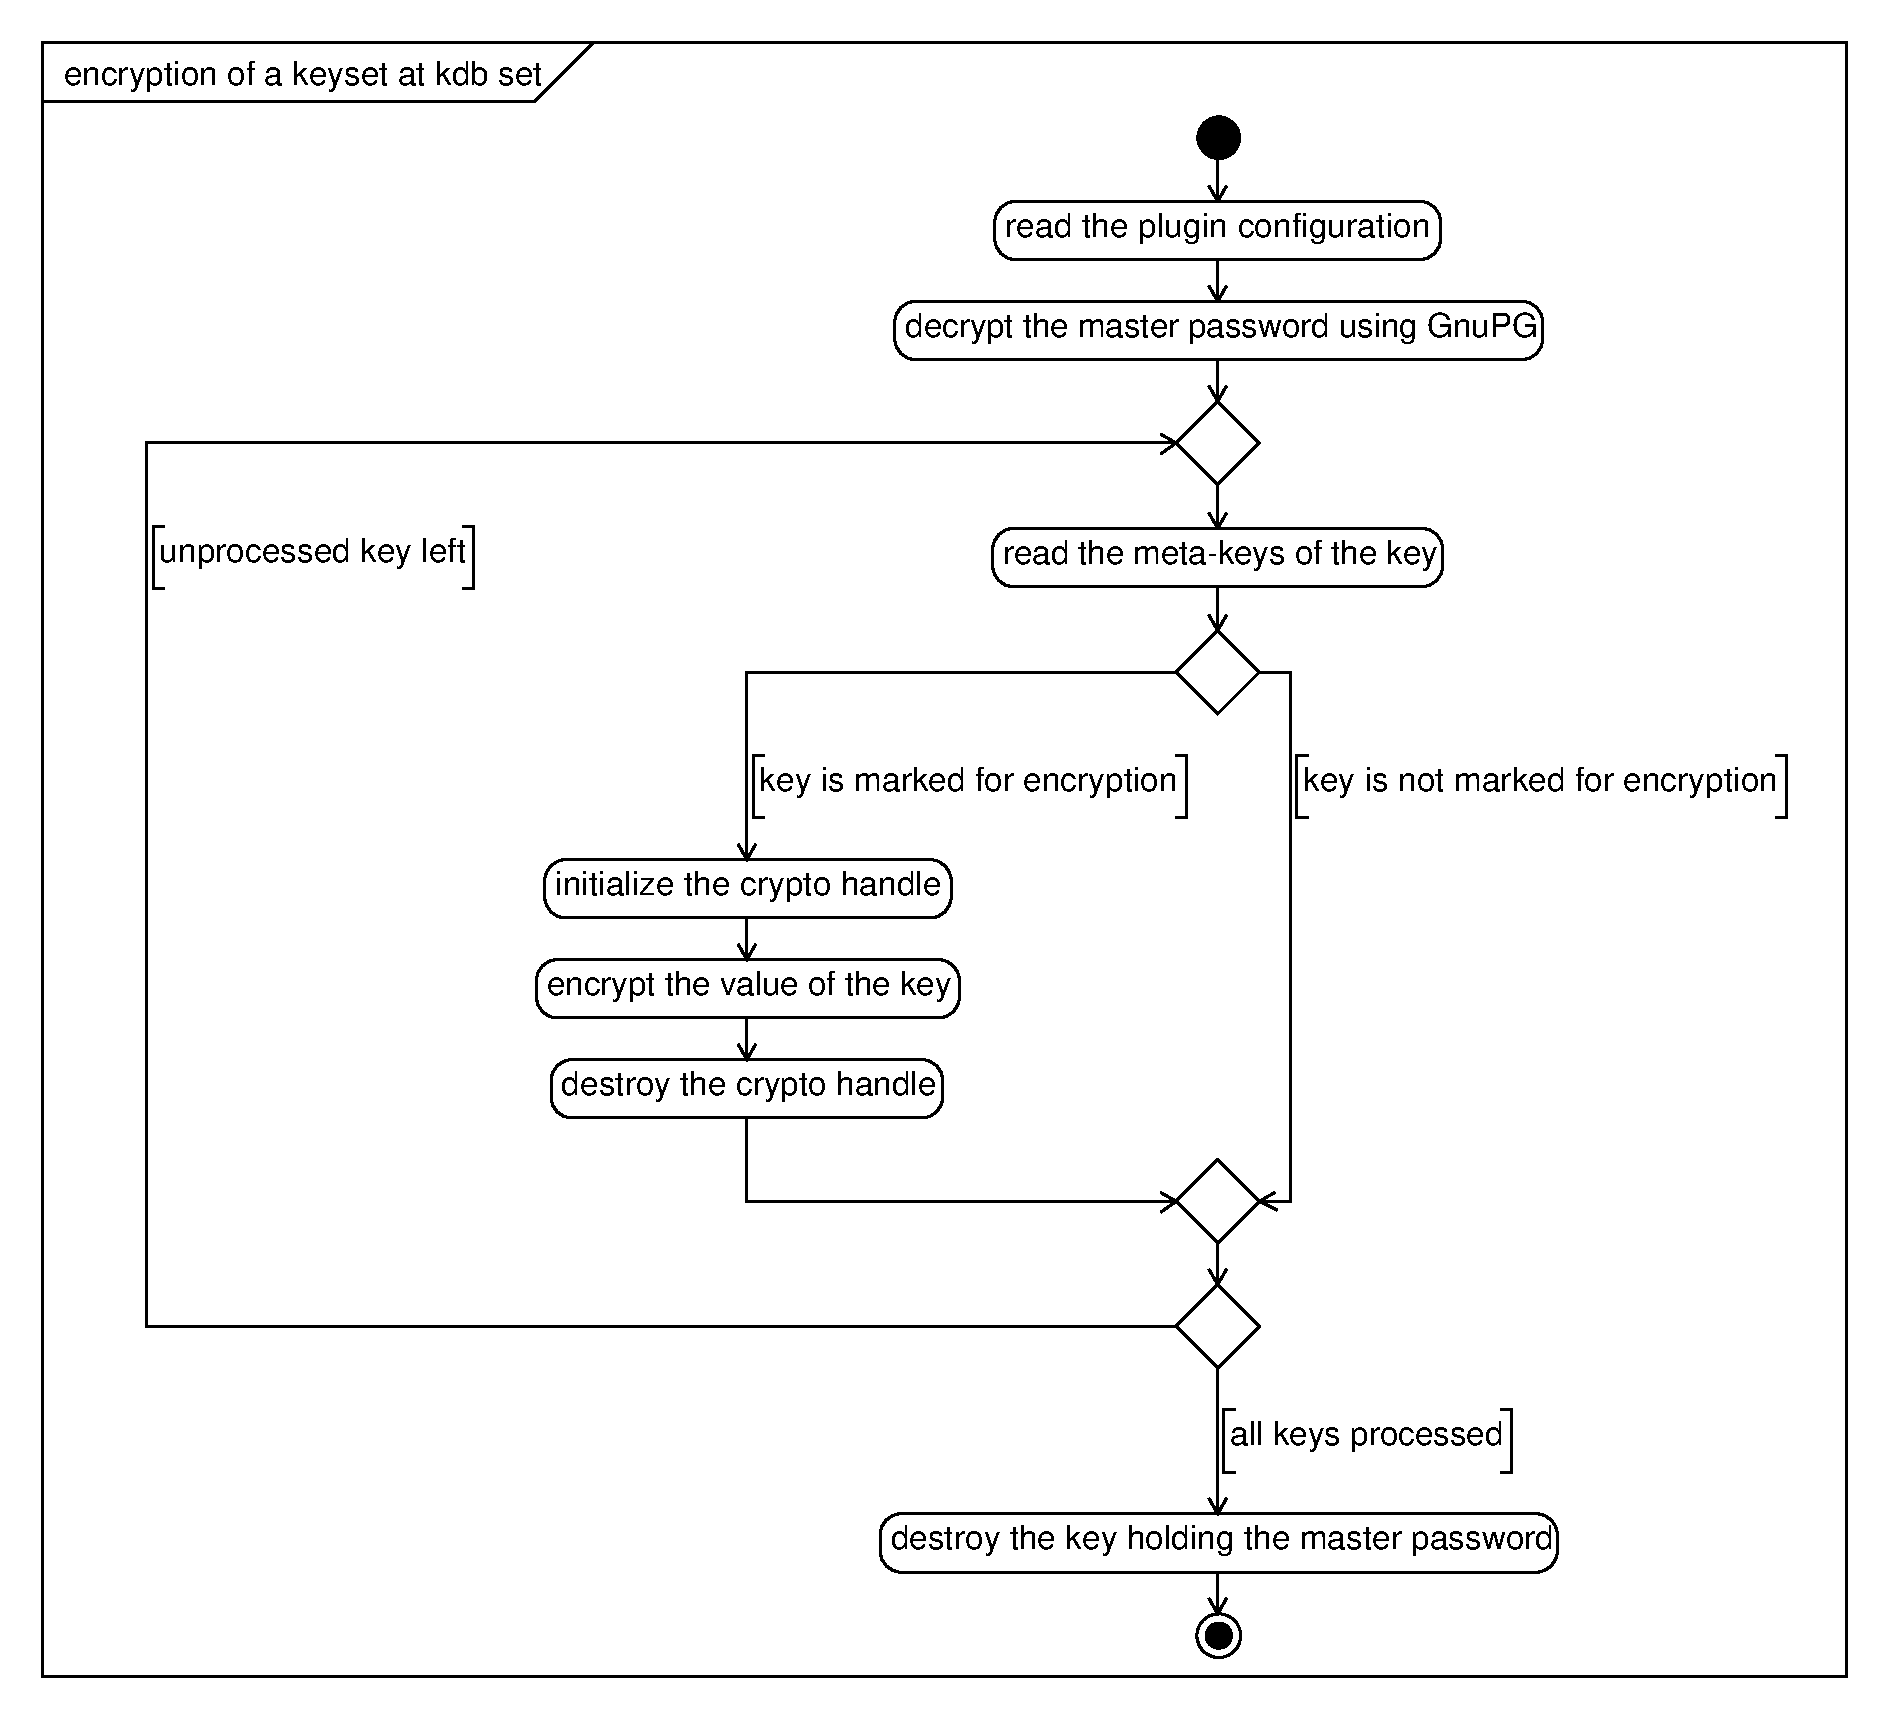
\includegraphics[width=15.0cm]{umlet-figures/impl_encrypt.pdf}
\end{figure}

\paragraph*{checkconf}
The \texttt{checkconf} method ensures that a master password is available in the plugin configuration of the \crypto.
If an encrypted master password is provided, a decryption run is started to see if the user owns the required GnuPG key.
Otherwise, a random master password is created, encrypted using GnuPG and stored in the plugin configuration.
The encryption key has to be specified within the plugin configuration.
If no such GnuPG private key is specified, the \crypto ~throws an error.

Figure \ref{impl_checkconf} on page \pageref{impl_checkconf} illustrates how the \texttt{checkconf} method works in detail.

\begin{figure}[h]
\center
\caption{Crypto Plugin: the kdb checkconf method}
\label{impl_checkconf}
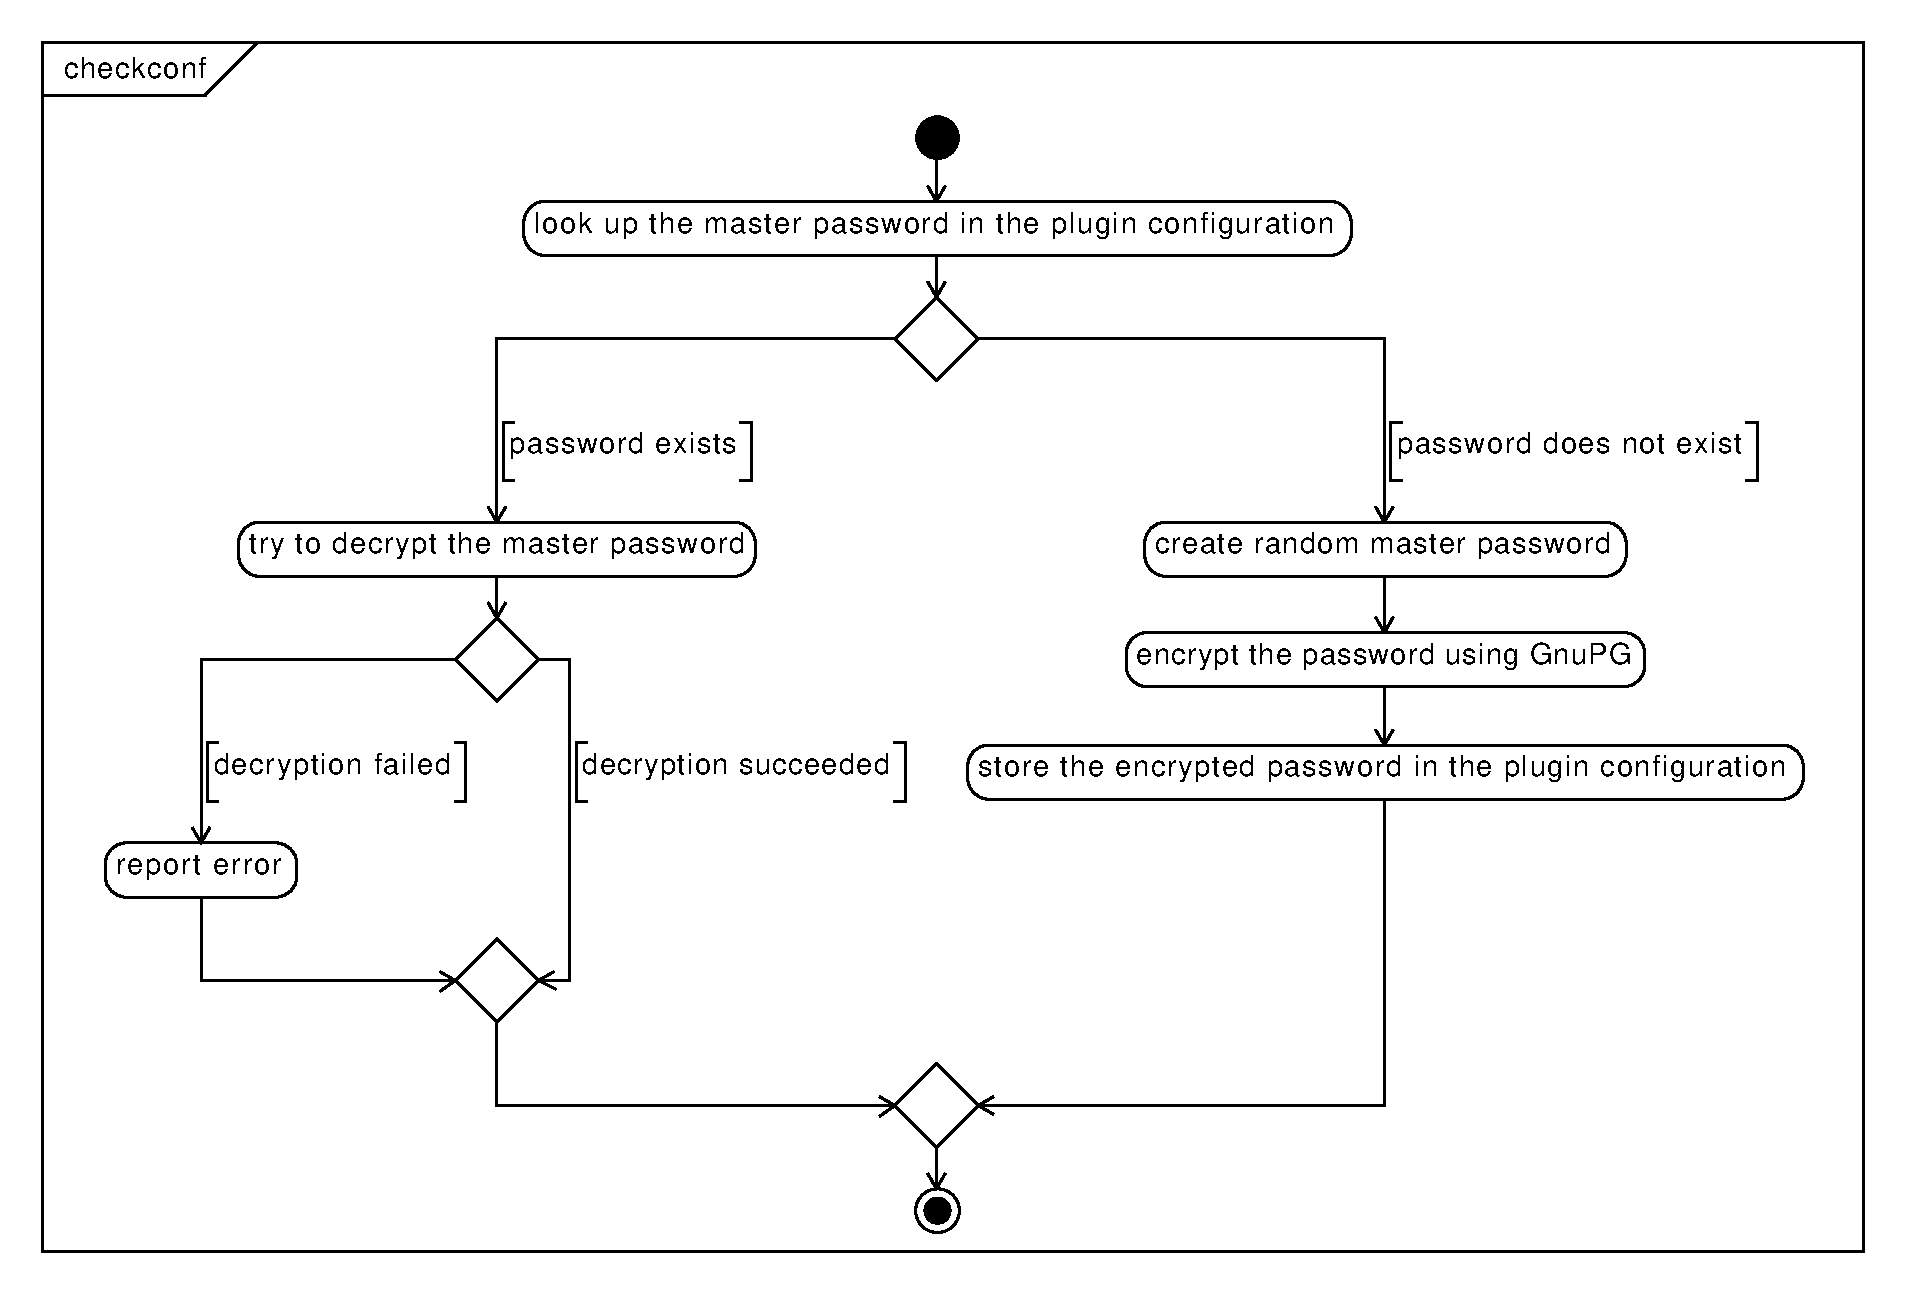
\includegraphics[width=15.0cm]{umlet-figures/impl_checkconf.pdf}
\end{figure}

\subsubsection{Compilation Variants}

For every provider of cryptographic functions (see Section \ref{intro-provider} on page \pageref{intro-provider}) a compilation variant of the \crypto ~is created.
The following compilation variants exist:
\begin{enumerate}
	\item \texttt{crypto\_botan} for the Botan library
	\item \texttt{crypto\_gcrypt} for libgcrypt
	\item \texttt{crypto\_openssl} for the OpenSSL library
\end{enumerate}

\subsection{Details About The Crypto Libraries}\label{details-about-the-crypto-libraries}



\section{Fcrypt Plugin}\label{fcrypt-plugin}

\subsection{Reasons For Developing The Plugin}

% crypto not good for entire config files -> too much overhead
% other performance benchmark -> GPG also uses libgcrypt

\subsection{Benefits for the Elektra Project}

% Users can encrypt entire configuration files
% no compile-time dependency which is nice for developers

\subsection{Challenges}

% Elektras internal API -> sync plugin workaround

\subsection{Technical Aspects}

% cryptographic operations are entirely handled by GnuPG


The \fcrypt{} was written to encrypt and decrypt whole files using the GPG interface mentioned before.
One of its advantages is that there are no dependencies at compile time.
Only the \texttt{gpg2} or \texttt{gpg} binaries are required as runtime dependency.

Again the GPG keys to be used for encryption are defined in the plugin configuration following the same semantics as the \crypto{}.


\section{Base64 Plugin}\label{base64-plugin}

% Chapter Outro

This chapter explained the Elektra plugin system and how we used it to introduce cryptographic methods to the Elektra project.
Now that we have an application to examine, we continue with the description of the actual measurements in the following chapter.
